\documentclass[conference]{IEEEtran}
% Packages
\usepackage{amsmath} % for mathematical equations
\usepackage{graphicx} % for including images
\usepackage{listings}
\usepackage{mathtools}

\begin{document}




% Title
\title{Final Project}
\author{John Carlsson & Lukas Runt}
\date{\today}



\maketitle

% Abstract
\begin{abstract}
The aim of the project was to solve two tasks. The first to identify how a certain network was generated
and the other to maximize the cumulative revenue obtained auctions over a marketing campaign. The results showed
that the network was generated using a configuration model with the degrees beeing normaly distributed around
23 with a standard deviation of 5. To maximize the cumulative revenue bla bla and bla was used
\end{abstract}

% Introduction
\section{Introduction}
This section introduces the tasks at hand.

\begin{itemize}
    \item Task1:\\ Consider the network N represented in the file net\_x, where x is your group number.
    This network has been generated with one of the network models seen during the course.
    You have to analyze the network N with the network mining tools (the ones shortlisted in the
    midterm project) and guess which model has been used for creating it. Your guess has to be
    supported by an appropriate set of experiments to confirm that networks generated with the
    proposed model have characteristics similar to N (note that you have to guess also the parameters of
    the model). \\

    \item Task2:\\ Your company is specialized in producing applications for social networks. You have been assigned
    the task of selling these applications with the goal of maximizing the revenue for the company. The
    contract between your company and the social network allows you to access to your preferred nodes
    over the network, and to spread whichever information you want from that node. However, the
    contract also constraints you to access to only one node every day. Then, your strategy is every day
    to select a node and spread from this node information about a network auction for selling k items
    (i.e., each day you start a different auction). Clearly, the information spreading process is not
    deterministic: in fact, even if a node invites a neighbor into the auction, it is not for sure that the
    latter will participate in the auction. We assume that the probability that a neighbor accepts to
    participate depends on the strength of the relationship among the two communicating nodes.
    Unfortunately, while you know the topology of the network, you do not know the strength of these
    relationships.\\ \\
    Hence, you have to choose every day the node from which to start a social network auction in order
    to maximize the cumulative revenue obtained by all the auctions over the entire campaign. To this
    aim you are required at each day to both be able to reach agents with large valuation about the items
    you are selling and to selects a kind of auction in order to maximize the amount of money that you
    are able to collect from them. Notice that you can use different types of auctions in different days.

\end{itemize}

% Methodology
\section{Task1}
This section describes the methodology used in task 1.

\subsection{Analysis}
First an analysis was made of the given network to see the overall structure. This was made with the NetworkX
library for python, where we quickly and easily can get some information about the graph.


The network has the following characteristics:
\begin{center}
    \begin{tabular}{|c|c|}
        
        \hline
        Number of nodes & 20 000 \\
        \hline
        Number of edges & 227739 \\
        \hline
        Directed? & False \\
        \hline
        Connected? & True \\
        \hline
    \end{tabular}

\end{center}

We see that the graph is one giant component that is undirected.


By looking at the distribution of neighbors we get the following graph.
\begin{figure}[h]
    \centering
    \caption{Number of neighbors}
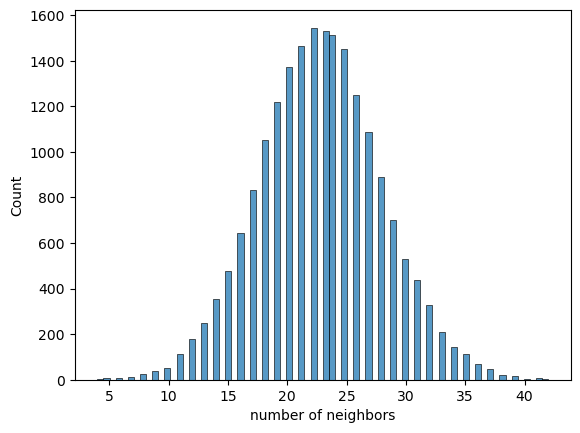
\includegraphics[scale = 0.55]{/Users/johncarlsson/Desktop/Social Network Analysis/final/figures/histo_facit.png}
\end{figure}

The number of neighbors that each node has gives us clues as to how the graph was constructed, if the degrees follow
a distribution, we know that a configuration model was used to construct the graph. So we plot the given graph and compare it
to some common distributions.

\begin{figure}[h]
    \centering
    \caption{Comparison of distributions}
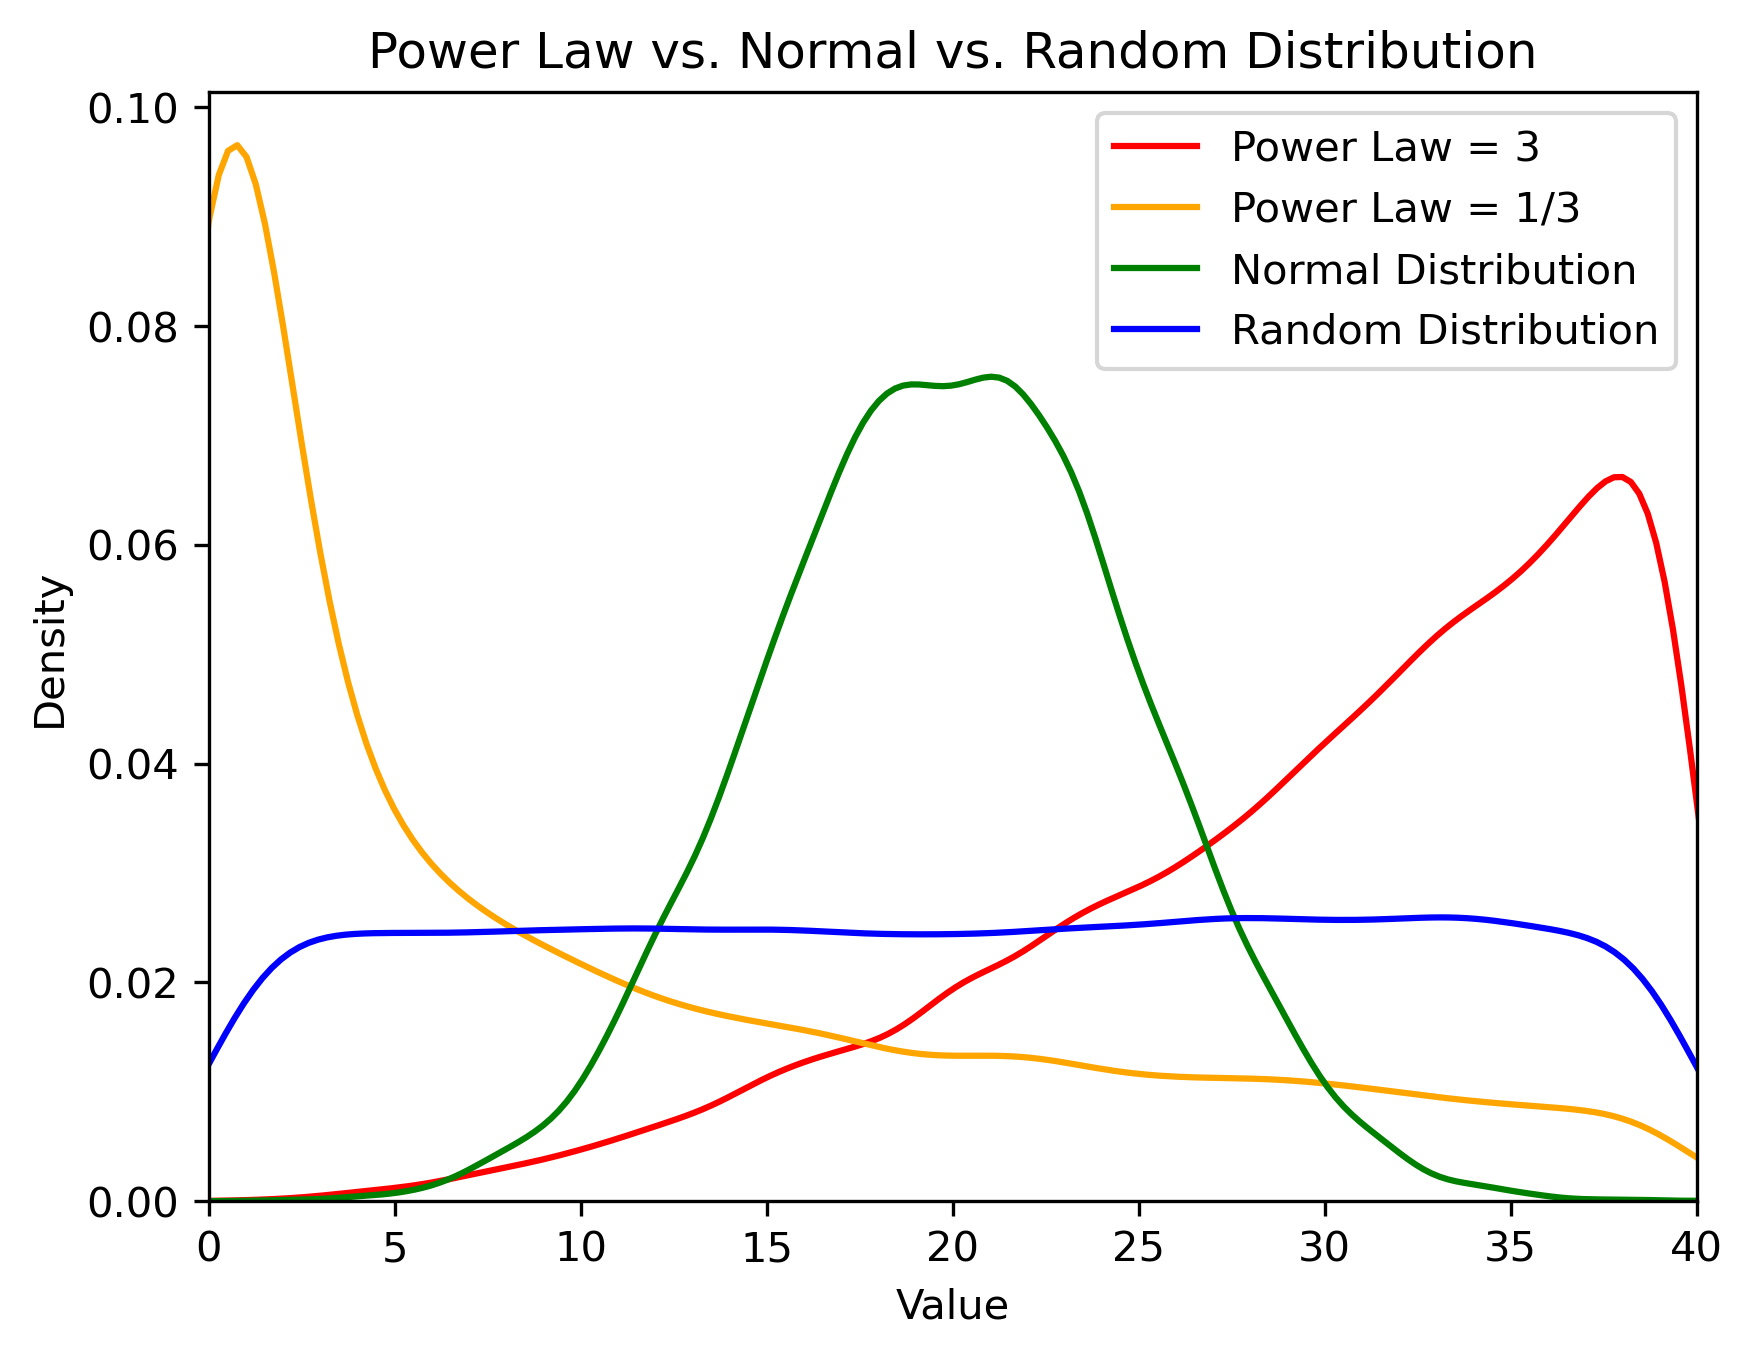
\includegraphics[scale = 0.55]{/Users/johncarlsson/Desktop/Social Network Analysis/final/figures/distribution_plot.png}
\end{figure}

\subsection[short]{Experiments}
Now that we know how the graph looks, can we replicate it? We from the prvious chapter that the graph strongly
ressembles a normal distribution and we can then use a configuration model to create a similar graph.
We can get the precise distribution and mean from the model which are 22.77 and 5.15.
By creating one hundred lists of degrees based these parameters and taking the average and creating a graph with 
a configuration model, we get the following graph of neighbour distribution.

\begin{figure}[h]
    \centering
    \caption{Number of neighbors expirimental graph}
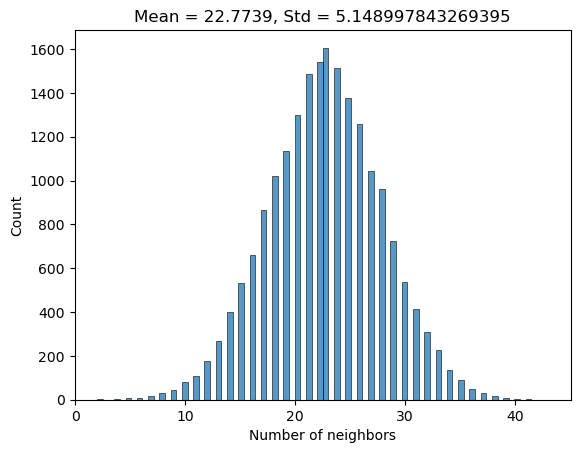
\includegraphics[scale = 0.55]{/Users/johncarlsson/Desktop/Social Network Analysis/final/figures/histo_fit.png}
\end{figure}

They are evidently very similar.

Now looking at connectivity and if the graph is directed. We get the same results as for the original graph.

by comparing different measures of centrality, here the min and max values are shown, we can see 
that the graphs are indeed very similar.

\begin{center}
    \begin{tabular}{|c|c|c|}
        
        \hline
        Centrality & Original network & Expirimental network \\
        \hline
        Degree & 0.2323 & 0.2323 \\
        \hline
        Closeness & 0.2323 & 0.2323 \\
        \hline
        Betweenness & 0.2323 & 0.2323 \\
        \hline
    \end{tabular}

\end{center}

% Results


\section{Task2}
This section describes the methodology used in task 2.

\subsection{Analysis}
First an analysis was made of implementing the VCG, MUDAR, and MUDAR algorithms and testing its gained revenue. We tested the algorithms on the assigned graph when we were picking the unsorted nodes. Then we try to improve the revenue by picking the sorted nodes by degree, centrality, or combination of more properties of the nodes and comparing them.  

\subsection{Experiments}
As we mentioned in the analysis we have tested all implemented methods with random picking nodes. We have tested it three times on time horizont 100000, k was randomly selected between 0,5\% to 5\% of nodes. We got the following average revenues per one-time horizont:

\begin{center}
	Comparing methods with a random choice of points
	\vspace{10pt}
   \begin{tabular}{|c|c|c|c|}
        \hline
        Attempt & VCG & MUDAN & MUDAR \\
        \hline
        1 & 159.161 & 38.904 & 147.700 \\
        \hline
        2 & 164.747 & 38.958 & 148.427 \\
        \hline
        3 & 168.952 & 40.045 & 148.356 \\
        \hline
    \end{tabular}

\end{center}

We can see that the most powerful algorithm with the biggest average revenue is the VCG algorithm followed by the MUDAR algorithm. The MUDAN algorithm gives really bad revenues. We can mention, that the revenue of the VCG algorithm depends on the amount of money donated for the report to the friend. We choose the revenue for reporting a friend to value 5. Value 10 was the average revenue of about 100 per time horizon, with revenue for report 1 being the average revenue of about 200. 

In the next experiment, we tested the improving impact of sorting the nodes by degree, centrality, and by combining both values. 

As the first improvement, we use sorting by the highest degree of the node.
\begin{center}
	Revenues after sorting nodes by degree
	\vspace{10pt}
   \begin{tabular}{|c|c|c|c|}
        \hline
        Attempt & VCG & MUDAN & MUDAR \\
        \hline
        1 & 179.515 & 40.818 & 166.346 \\
        \hline
        2 & 175.252 & 40.694 & 165.626 \\
        \hline
        3 & 175.186 & 40.827 & 164.436 \\
        \hline
    \end{tabular}
\end{center}

We can see that revenues were slightly improved. In the next case, we tried sorting nodes by centrality.

 \begin{center}
	Revenues after sorting nodes by centrality
	\vspace{10pt}
   \begin{tabular}{|c|c|c|c|}
        \hline
        Attempt & VCG & MUDAN & MUDAR \\
        \hline
        1 & 181.819 & 41.268 & 155.774 \\
        \hline
        2 & 178.263 & 41.624 & 160.985 \\
        \hline
        3 & 177.412 & 41.305 & 163.764 \\
        \hline
    \end{tabular}
\end{center}

In this case, we can see small improvements in VCG and MUDAN algorithms, but also a small degradation of revenue in the Mudar algorithm.
What if we will put both these sorting together? In the next case, we have just sorted the nodes by combining the centrality and degree of the node. We created this metric by multiplying the centrality and degree. The results were as follows:

 \begin{center}
	Revenues after sorting nodes by combination
	\vspace{10pt}
   \begin{tabular}{|c|c|c|c|}
        \hline
        Attempt & VCG & MUDAN & MUDAR \\
        \hline
        1 & 178.239 & 42.328 & 168.326 \\
        \hline
        2 & 181.961 & 41.205 & 171.417 \\
        \hline
        3 & 180.715 & 41.072 & 167.209 \\
        \hline
    \end{tabular}
\end{center}
	
The results were improved very little except in the Mudar, where the improvement is obvious. The behavior seems more stable than without the combination. 

\section{Results & Conclusion}
This section presents the results of the project.

\subsection[short]{Task 1}
Based on the previous chapter, we believe that the network was created by using a configuration model.
The parameters for the model was the following:

\begin{center}
    \begin{tabular}{|c|c|}
        \hline
        Parameter & Value \\
        \hline
        Nodes & 20000 \\
        \hline
        Degree & \sim \mathcal{N}(\mu,\,\sigma^{2}) \\
        \hline
        \mu & 23 \\
        \hline
        \sigma & 5\\
        \hline
        
    \end{tabular}

\end{center}

Degree is a list containing the number of neighbors for each node.

\subsection[short]{Task 2}
Based on the previous chapter, the VGC and Mudar auctions give comparable results. Mudan gives really poor revenues. In the next part, we have tried to maximalize the revenue by picking the best nodes. The best result proved to be combining centrality and degree.

\end{document}